\setcounter{section}{1}
\section{BẢNG TẦN SỐ TƯƠNG ĐỐI VÀ BIỂU ĐỒ TẦN SỐ TƯƠNG ĐỐI}
%%%%%%%%%%%%%%%%
\subsection{Trọng tâm kiến thức}%Tên bài
\begin{tomtat}
	\subsubsection{Bảng tần số tương đối}
	\begin{boxdn}
		Tần số tương đối của một giá trị $x$ trong mẫu dữ liệu được tính theo công thức $f=\dfrac{m}{N}\cdot 100\%$ trong đó $m$ là tần số của $x$ và $N$ là cỡ mẫu.\\
		Bảng tần số tương đối biểu diễn tần số tương đối của mỗi giá trị trong mẫu dữ liệu.\\
		Bảng gồm hai dòng (hoặc hai cột), dòng (hoặc cột) thứ nhất ghi các giá trị khác nhau của mẫu dữ liệu, dòng (hoặc cột) thứ hai ghi các tần số tương đối tương ứng với mỗi giá trị đó.
	\end{boxdn}
	\begin{nx}
		Bảng tần số tương đối giúp chúng ta nhanh chóng quan sát được đặc điểm của mẫu dữ liệu như tần số tương đối của mỗi giá trị, giá trị xuất hiện thường xuyên nhất, giá trị xuất hiện ít thường xuyên nhất, ... Bảng tần số tương đối cũng giúp chúng ta so sánh mức độ xuất hiện thường xuyên của một giá trị trong nhiều mẫu số liệu khác nhau.
	\end{nx}
	\begin{note}
		\hfill
		\begin{itemize}
			\item Tổng tần số tương đối của tất cả các giá trị luôn bằng $100\%$.
			\item Có thể ghép bảng tần số và bảng tần số tương đối thành bảng tần số - tần số tương đối như sau
		\end{itemize}
	\begin{table}[h!]
		\centering
		\begin{tabular}{|c|c|c|c|c|c|c|}
			\hline
Số lỗi chính tả & $0$ & $1$  & $2$  & $3$  & $4$  & $5$  \\ \hline
Tần số & $4$ & $10$ & $7$  & $5$  & $8$  & $6$  \\ \hline
Tần số tương đối  & $10,0\%$ & $25,0\%$ & $17,5\%$ & $12,5\%$ & $20,0\%$ & $15,0\%$ \\ \hline
		\end{tabular}
	\end{table}
	\end{note}
	%%==========Ví dụ 1
	\begin{vd}%[Dự án EX-9-Đề Cương Toán 9]%[Trần Vinh]%[9D5N2-1]
	Bạn Linh gieo một con xúc xắc cân đối và đồng chất một số lần và ghi lại tần số tương đối số lần xuất hiện của mỗi mặt trong bảng thống kê sau:
	\begin{center}
		\begin{tabular}{|c|c|c|c|c|c|c|}
			\hline Mặt & $1$ chấm & $2$ chấm & $3$ chấm & $4$ chấm & $5$ chấm & $6$ chấm \\
			\hline Tần số tương đối & $15\%$ & $18\%$ & $12\%$ & $21\%$ & $16\%$ & $13\%$ \\
			\hline
		\end{tabular}
	\end{center}
	Số liệu trong bảng tần số tương đối trên có hợp lí không? Tại sao?
	\loigiai{
		Ta có: $15\%+18\%+12\%+21\%+16\%+13\%=95\%$.\\
		Như vậy, số liệu trong bảng tần số tương đối là không hợp lí vì tổng tần số tương đối của tất cả các giá trị nhỏ hơn $100\%$.}
	\end{vd}
%%==========Ví dụ 2
\begin{vd}%[Dự án EX-9-Đề Cương Toán 9]%[Trần Vinh]%[9D5N2-1]
Một lớp học có $30$ học sinh được khảo sát về số anh chị em ruột. Kết quả thu được như sau:
\begin{center}
	\begin{tabular}{|c|c|c|c|c|}
		\hline
		Số anh chị em & $0$ & $1$ & $2$ & $3$ \\ \hline
		Tần số & $6$ & $12$ & $9$ & $3$ \\ \hline
	\end{tabular}
\end{center}
Hãy lập bảng tần số tương đối (làm tròn đến $1\%$).
\loigiai{
Tổng số học sinh là $6 + 12 + 9 + 3 = 30$.\\
Số em học sinh không có anh chị em là $6$ nên tần số tương đối là $f_{1}=\dfrac{6}{30}=20\%$.\\
Số em học sinh có $1$ anh chị em là $12$ nên tần số tương đối là $f_{2}=\dfrac{12}{30}=40\%$.\\
Số em học sinh có $2$ anh chị em là $9$ nên tần số tương đối là $f_{3}=\dfrac{9}{30}=30\%$.\\
Số em học sinh có $3$ anh chị em là $3$ nên tần số tương đối là $f_{4}=\dfrac{3}{30}=10\%$.\\
Ta có bảng tần số tương đối như sau
\begin{center}
	\begin{tabular}{|c|c|c|c|c|}
		\hline
		Số anh chị em & $0$ & $1$ & $2$ & $3$ \\ \hline
		Tần số tương đối & $20\%$ & $40\%$ & $30\%$ & $10\%$ \\ \hline
	\end{tabular}
\end{center}
Tổng tần số tương đối là $100\%$, bảng này hợp lý.
}
\end{vd}
\end{tomtat}
%%%%%%%%%%%%%%%%%
\subsection{BÀI TẬP VẬN DỤNG}
%============================
\begin{dang}{Lập bảng tần số tương đối và một số yếu tố liên quan}
\end{dang}
%%==========Bài tập 1
\begin{bt}%[Dự án EX-9-Đề Cương Toán 9]%[Trần Vinh]%[9D5N2-1]
	Sau bài thi môn Ngữ văn, cô giáo ghi lại số lỗi chính tả mà một số học sinh mắc phải vào bảng thống kê sau
	\begin{center}
		\begin{tabular}{|l|l|l|l|l|l|l|l|l|l|l|l|l|l|l|l|l|l|l|l|}
			\hline $2$& $5$& $2$& $2$& $1$& $3$& $4$& $0$& $5$& $2$& $5$& $1$& $2$& $1$& $3$& $5$& $1$& $0$& $4$& $1$\\
			\hline $4$& $2$& $1$& $4$& $3$& $3$& $2$& $0$& $4$& $5$& $4$& $5$& $1$& $4$& $1$& $1$& $0$& $3$& $1$& $4$\\
			\hline
		\end{tabular}
	\end{center}
		\begin{enumerate}
		\item Mẫu số liệu trên gồm những giá trị khác nhau nào?
		\item Hãy lập bảng tần số và bảng tần số tương đối của số lỗi chính tả mà học sinh mắc phải.
		\item Trong số học sinh được khảo sát, cô giáo muốn chọn ra $35\%$ số học sinh mắc nhiều lỗi nhất. Hỏi cô giáo cần chọn các học sinh mắc bao nhiêu lỗi?
	\end{enumerate}
	\loigiai{
			\begin{enumerate}
			\item Các giá trị khác nhau của mẫu số liệu là $0$; $1$; $2$; $3$; $4$; $5$.
			\item Kích thước mẫu $N=40$.\\
			Bảng tần số
			\begin{center}
				\begin{tabular}{|c|c|c|c|c|c|c|}
					\hline Số lỗi chính tả & $0$& $1$& $2$& $3$& $4$& $5$\\
					\hline Tần số & $4 $& $10$& $7$& $5$& $8$& $6$\\
					\hline
				\end{tabular}
			\end{center}
			Vì tần số của giá trị $0$ là $4$ nên tần số tương đối của giá trị $0$ là $\dfrac{4}{40}\cdot100\%=10{,}0\%$.\\
			Vì tần số của giá trị $1$ là $10$ nên tần số tương đối của giá trị $1$ là $\dfrac{10}{40}\cdot100\%=25{,}0\%$.\\
			Tương tự, ta tính được tần số tương đối của các giá trị $2$; $3$; $4$; $5$ lần lượt là $17{,}5\%$; $12{,}5\%$; $20{,}0\%$; $15{,}0\%$.\\
			Ta thu được bảng tần số tương đối như sau
			\begin{center}
				\begin{tabular}{|c|c|c|c|c|c|c|}
					\hline Số lỗi chính tả & $0$ & $1$ & $2$ & $3$ & $4$ & $5$ \\
					\hline Tần số tương đối & $10{,}0\%$ & $25{,}0\%$ & $17{,}5\%$ & $12{,}5\%$ & $20{,}0\%$ & $15{,}0\%$ \\
					\hline
				\end{tabular}
			\end{center}
			\item Vì $20{,}0\%+15{,}0\%=35\%$ nên cô giáo cần chọn các bạn mắc $4$ lỗi hoặc $5$ lỗi.
		\end{enumerate}
	}
\end{bt}
%%==========Bài tập 2
\begin{bt}%[Dự án EX-9-Đề Cương Toán 9]%[Trần Vinh]%[9D5H2-1]
		\begin{enumerate}
		\item
		Tại một trại hè thanh thiếu niên quốc tế, người ta tìm hiểu xem mỗi đại biểu tham dự có thể sử dụng được bao nhiêu ngoại ngữ. Kết quả được biểu diễn như bảng sau
		\begin{center}
			\begin{tabular}{|c|c|c|c|c|c|}
				\hline Số ngoại ngữ & $1$ & $2$ & $3$ & $4$ & $\geq5 $ \\
				\hline Số đại biểu & $84$ & $64$ & $24$ & $16$ & $12$ \\
				\hline
			\end{tabular}
		\end{center}
		Hãy lập bảng tần số tương đối cho bài toán trên?
		\item Tại trại hè thanh thiếu niên quốc tế tổ chức một năm trước đó, có $54$ trong tổng số $220$ đại biểu tham dự có thể sử dụng được từ $3$ ngoại ngữ trở lên. Có ý kiến cho rằng: \lq\lq Tỉ lệ đại biểu sử dụng được từ $3$ ngoại ngữ trở lên có tăng giữa hai năm đó\rq\rq. Ý kiến đó đúng hay sai? Giải thích.
	\end{enumerate}
	\loigiai{
			\begin{enumerate}
			\item Ta có bảng tần số tương đối sau
			\begin{center}
				\begin{tabular}{|c|c|c|c|c|c|}
					\hline Số ngoại ngữ & $1$ & $2$ & $3$ & $4$ & $\geq5$ \\
					\hline Tần số & $84$ & $64$ & $24$ & $16$ & $12$ \\
					\hline Tần số tương đối & $42\%$ & $32\%$ & $12\%$ & $8\%$ & $6\%$ \\
					\hline
				\end{tabular}
			\end{center}
			\item Số đại biểu sử dụng được từ $3$ ngôn ngữ trở lên của năm nay là $24+16+12=52$.\\
			TỈ lệ đại biểu sử dụng được từ $3$ ngôn ngữ trở lên của năm nay là $\dfrac{52}{200}=0{,}26$.\\
			Tỉ lệ đại biểu sử dụng được từ $3$ ngôn ngữ trở lên của năm trước là $\dfrac{54}{220}=\dfrac{27}{110}\approx 0{,}23$.\\
			Do đó, ý kiến trên là đúng, vì $0{,}26>0{,}23$.
		\end{enumerate}
	}
\end{bt}
%%==========Bài tập 3
\begin{bt}%[Dự án EX-9-Đề Cương Toán 9]%[Trần Vinh]%[9D5N2-1]
	Thu thập dữ liệu về chất lượng không khí tại một địa điểm trong $30$ ngày mùa xuân cho kết quả như sau
	\begin{center}
		\begin{tabular}{llllllllll}
			M1, &M1, &M2, &M2, &M2, &M2, &M1, &M2, &M2, &M2,\\
			M2, &M2, &M2, &M2, &M2, &M4, &M3, &M3, &M3, &M3,\\
			M4, &M4, &M1, &M1, &M1, &M1, &M3, &M3, &M3, &M1.
		\end{tabular}
	\end{center}
	\begin{center}
		{\it (M1: Tốt;\quad M2: Trung bình;\quad M3: Kém;\quad M4: Xấu)}
	\end{center}
		\begin{enumerate}
		\item Lập bảng tần số tương đối cho dãy dữ liệu trên.
		\item Trong một ngày xuân, khả năng cao nhất địa điểm này có chất lượng không khí ở mức nào?
	\end{enumerate}
	\loigiai{	\begin{enumerate}
			\item Tổng số quan sát là $N=30$.\\
			Số ngày có chất lượng không khí ở các mức M1, M2, M3, M4 tương ứng là $m_1=8$, $m_2=12$, $m_3=7$, $m_4=3$.\\
			Do đó các tần số tương đối cho các mức M1, M2, M3, M4 lần lượt là
			$$
			f_1=\dfrac{8}{30}\approx26{,}7\%;\quad f_2=\dfrac{12}{30}=40 \%;\quad f_3=\dfrac{7}{30}\approx 23{,}3\%;\quad f_4=\dfrac{3}{30}=10\%.$$
			Ta có bảng tần số tương đối sau
			\begin{center}
				\begin{tabular}{|p{5cm}|p{2cm}|p{2cm}|p{2cm}|p{2cm}|}
					\hline Chất lượng không khí &\centering\arraybackslash M1 &\centering\arraybackslash M2 &\centering\arraybackslash M3 &\centering\arraybackslash M4 \\
					\hline Tần số tương đối &\centering\arraybackslash $26{,}7\%$ &\centering\arraybackslash $40\%$ &\centering\arraybackslash $23{,}3\%$ &\centering\arraybackslash $10\%$ \\
					\hline
				\end{tabular}
			\end{center}
			\item Trong một ngày xuân, khả năng cao nhất là địa điểm này có chất lượng không khí ở mức M2, tức là mức Trung bình.
	\end{enumerate}}
\end{bt}
%%==========Bài tập 4
\begin{bt}%[Dự án EX-9-Đề Cương Toán 9]%[Trần Vinh]%[9D5N2-1]
	\immini{Quay $50$ lần một tấm bìa hình tròn được chia thành ba hình quạt với các màu xanh, đỏ, vàng. Quan sát và ghi lại mũi tên chỉ vào hình quạt có màu nào khi tấm bìa dừng lại. Kết quả thu được như sau
		\begin{tabular}{ll}
			Xanh: &
			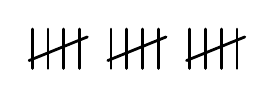
\begin{tikzpicture}[>=stealth,line join=round,line cap=round,font=\footnotesize,xscale=.2,yscale=.5]
				\foreach \i in {1,2,3,4}{
					\draw[line width=1pt] (\i,0)--(\i,1);
				}
				\draw[line width=1pt] (0.8,.2)--(4.5,.8);
				\foreach \i in {6,7,8,9}{
					\draw[line width=1pt] (\i,0)--(\i,1);
				}
				\draw[line width=1pt] (5.8,.2)--(9.5,.8);
				\foreach \i in {11,12,13,14}{
					\draw[line width=1pt] (\i,0)--(\i,1);
				}
				\draw[line width=1pt] (10.8,.2)--(14.5,.8);
			\end{tikzpicture}\\
			Đỏ: &
			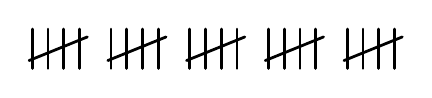
\begin{tikzpicture}[>=stealth,line join=round,line cap=round,font=\footnotesize,xscale=.2,yscale=.5]
				\foreach \i in {1,2,3,4}{
					\draw[line width=1pt] (\i,0)--(\i,1);
				}
				\draw[line width=1pt] (0.8,.2)--(4.5,.8);
				\foreach \i in {6,7,8,9}{
					\draw[line width=1pt] (\i,0)--(\i,1);
				}
				\draw[line width=1pt] (5.8,.2)--(9.5,.8);
				\foreach \i in {11,12,13,14}{
					\draw[line width=1pt] (\i,0)--(\i,1);
				}
				\draw[line width=1pt] (10.8,.2)--(14.5,.8);
				\foreach \i in {16,17,18,19}{
					\draw[line width=1pt] (\i,0)--(\i,1);
				}
				\draw[line width=1pt] (15.8,.2)--(19.5,.8);
				\foreach \i in {21,22,23,24}{
					\draw[line width=1pt] (\i,0)--(\i,1);
				}
				\draw[line width=1pt] (20.8,.2)--(24.5,.8);
			\end{tikzpicture}\\
			Vàng: &
			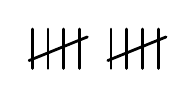
\begin{tikzpicture}[>=stealth,line join=round,line cap=round,font=\footnotesize,xscale=.2,yscale=.5]
				\foreach \i in {1,2,3,4}{
					\draw[line width=1pt] (\i,0)--(\i,1);
				}
				\draw[line width=1pt] (0.8,.2)--(4.5,.8);
				\foreach \i in {6,7,8,9}{
					\draw[line width=1pt] (\i,0)--(\i,1);
				}
				\draw[line width=1pt] (5.8,.2)--(9.5,.8);
			\end{tikzpicture}
		\end{tabular}
	}{
		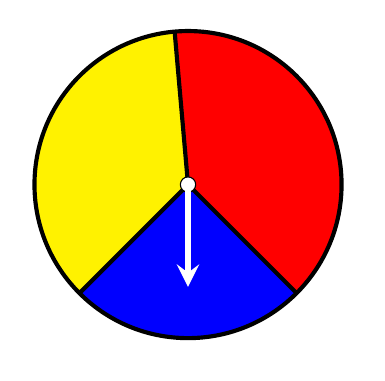
\begin{tikzpicture}[>=stealth,line join=round,line cap=round,font=\footnotesize,scale=0.65]
			\draw (0,0) coordinate (O)
			(O)++(95:3) coordinate (A)
			(O)++(-135:3) coordinate (B)
			(O)++(-45:3) coordinate (C)
			;
			\fill[red] (O)--(C) arc (-45:95:3 cm)--(O);
			\fill[yellow] (O)--(A) arc (95:225:3 cm)--(O);
			\fill[blue] (O)--(B) arc (-135:-45:3 cm)--(O);
			\draw[line width=1.5pt] (O) circle (3cm) (O)--(A) (O)--(B) (O)--(C);
			\draw[fill=white] (O) circle (1.5mm);
			\draw[white,->,line width=2.5pt] (O)--(0,-2);
		\end{tikzpicture}
	}
		\begin{enumerate}
		\item Lập bảng tần số tương đối cho kết quả thu được.
		\item Ước lượng xác suất mũi tên chỉ vào hình quạt màu đỏ.
	\end{enumerate}
	\loigiai{
			\begin{enumerate}
			\item Số lần xuất hiện màu Xanh, Đỏ, Vàng tương ứng là $m_1=15$, $m_2=25$, $m_3=10$.\\
			Do đó, các tần số tương đối cho các màu Xanh, Đỏ, Vàng lần lượt là
			$$f_1=\dfrac{15}{50}=30\%;\quad f_2=\dfrac{25}{50}=50\%;\quad f_3=\dfrac{10}{50}=20\%.$$
			Ta có bảng tần số tương đối như sau:
			\begin{center}
				\begin{tabular}{|p{4cm}|p{2cm}|p{2cm}|p{2cm}|}
					\hline Màu &\centering\arraybackslash Xanh &\centering\arraybackslash Đỏ &\centering\arraybackslash Vàng\\
					\hline Tần số tương đối &\centering\arraybackslash $30\%$ &\centering\arraybackslash $50\%$ &\centering\arraybackslash $20\%$\\
					\hline
				\end{tabular}
			\end{center}
			\item Vì tần số tương đối của màu đỏ là $50\%$ nên ước lượng xác suất mũi tên chỉ vào hình quạt màu đỏ là $50\%$.
		\end{enumerate}
	}
\end{bt}
%%==========Bài tập 5
\begin{bt}%[Dự án EX-9-Đề Cương Toán 9]%[Trần Vinh]%[9D5N2-1]
	Trong tác phẩm \lq\lq \textit{Truyện Kiều}\rq\rq\, bất hủ của nhà thơ Nguyễn Du có hai câu thơ
	\begin{center}
		\lq\lq \textit{Dưới trăng quyên đã gọi hè \\
			Đầu tường lửa lựu lập lòe đơm bông}\rq\rq
	\end{center}
	Mẫu dữ liệu thống kê các chữ cái G; L; N; T lần lượt xuất hiện trong hai câu thơ trên là
	\begin{center}
		\begin{tabular}{|cccccccccccccc|}
			\hline 	T &N &G &N &G &T &N &G &L &L &L &L &N &G\\
			\hline
		\end{tabular}
	\end{center}
	Lập bảng tần số tương đối của mẫu dữ liệu thống kê đó.
	\loigiai{
		Mẫu dữ liệu thống kê đó có $14$ dữ liệu ($N=14$) và có $4$ giá trị khác nhau là G; L; N; T.\\
		Các giá trị G; L; N; T lần lượt có tần số, tần số tương đối là $n_1=4$; $n_2=4$; $n_3=4$; $n_4=2$;
		\begin{multicols}{2}
			\begin{itemize}
				\item $f_1=\dfrac{4\cdot100}{14}\%\approx28{,}57\%$;
				\item $f_2=\dfrac{4\cdot100}{14}\%\approx28{,}57\%$;
				\item $f_3=\dfrac{4\cdot100}{14}\%\approx28{,}57\%$;
				\item $f_4=\dfrac{2\cdot100}{14}\%\approx14{,}29\%$.
			\end{itemize}
		\end{multicols}
		Bảng tần số tương đối của mẫu dữ liệu thống kê trên là
		\begin{center}
			\begin{tabular}{|>{\centering\arraybackslash}m{4cm}|>{\centering\arraybackslash}m{1.5cm}|>{\centering\arraybackslash}m{1.5cm}|>{\centering\arraybackslash}m{1.5cm}|>{\centering\arraybackslash}m{1.5cm}|>{\centering\arraybackslash}m{1.5cm}|}
				\hline 	Chữ cái $(x)$	&G	&L	&N	&T	&Cộng \\
				\hline	Tần số tương đối $(\%)$	&$28{,}57\%$ &$28{,}57\%$ &$28{,}57\%$ &$14{,}29\%$ &$100\%$ \\
				\hline
			\end{tabular}
		\end{center}
	}
\end{bt}
%%==========Bài tập 6
\begin{bt}%[Dự án EX-9-Đề Cương Toán 9]%[Trần Vinh]%[9D5N2-1]
	Sau khi điều tra $60$ hộ gia đình tại một vùng dân cư về số nhân khẩu của mỗi hộ gia đình, người ta được dãy số liệu thống kê (hay còn gọi là mẫu số liệu thống kê) như sau
	\begin{center}
		\begin{tabular}{|cccccccccccccccccccc|}
			\hline
			$6$	&$6$ &$6$ &$7$ &$5$ &$5$ &$4$ &$5$ &$6$ &$4$ &$4$ &$8$ &$6$ &$6$ &$6$ &$6$ &$5$ &$5$ &$5$ &$4$ \\
			$6$ &$6$ &$7$ &$7$ &$5$ &$5$ &$5$ &$5$ &$6$ &$4$ &$4$ &$6$ &$6$ &$6$ &$6$ &$6$ &$5$ &$5$ &$5$ &$4$ \\
			$8$	&$6$ &$6$ &$5$ &$5$ &$5$ &$5$ &$6$ &$6$ &$4$ &$5$ &$6$ &$7$ &$6$ &$8$ &$6$ &$5$ &$5$ &$6$ &$5$ \\
			\hline
		\end{tabular}
	\end{center}
	Lập bảng tần số tương đối của mẫu số liệu thống kê trên.
	\loigiai{
		Mẫu dữ liệu thống kê có $60$ dữ liệu ($N=60$) và có $5$ giá trị khác nhau là $4$, $5$, $6$, $7$, $8$.\\
		Tần số là $n_1=8$; $n_2=21$; $n_3=24$; $n_4=4$; $n_5=3$.\\
		Tần số tương đối là
			\begin{itemize}
				\item $f_1=\dfrac{8\cdot100}{60}\%\approx13{,}33\%$;
				\item $f_2=\dfrac{21\cdot100}{60}\%=35\%$;
				\item $f_3=\dfrac{24\cdot100}{60}\%=40\%$;
				\item $f_4=\dfrac{4 \cdot 100}{60} \%\approx6{,}67\%$;
				\item $f_5=\dfrac{3\cdot100}{60}\%=5\%$.
			\end{itemize}
		Bảng tần số tương đối của mẫu dữ liệu thống kê trên là
		\begin{center}
			\begin{tabular}{|>{\centering\arraybackslash}m{4cm}|>{\centering\arraybackslash}m{1.5cm}|>{\centering\arraybackslash}m{1.5cm}|>{\centering\arraybackslash}m{1.5cm}|>{\centering\arraybackslash}m{1.5cm}|>{\centering\arraybackslash}m{1.5cm}|>{\centering\arraybackslash}m{1.5cm}|}
				\hline 	Số nhân khẩu $(x)$	&$4$	&$5$	&$6$	&$7$	&$8$	&Cộng \\
				\hline	Tần số tương đối $(\%)$	&$13{,}33\%$ &$35\%$ &$40\%$ &$6{,}67\%$	&$5\%$ &$100\%$ \\
				\hline
			\end{tabular}
		\end{center}
	}
\end{bt}
%%==========Bài tập 7
\begin{bt}%[Dự án EX-9-Đề Cương Toán 9]%[Trần Vinh]%[9D5N2-1]
	Câu lạc bộ mĩ thuật của nhà văn hoá thiếu nhi thống kê tuổi của các thành viên lớp hội hoạ và biểu diễn dữ liệu qua bảng sau
	\begin{center}
		Tuổi của các thành viên lớp hội hoạ\\
		\begin{tabular}{|l|c|c|c|c|c|c|c|}
			\hline
			Tuổi & $9$ & $10$ & $11$ & $12$ & $13$ & $14$ & Tổng\\
			\hline
			Tần số & $10$ & $4$ & $6$ & $2$ & $12$ & $6$ & $N=40$\\
			\hline
		\end{tabular}
	\end{center}
	Tính tần số tương đối của mỗi giá trị và lập bảng tần số tương đối.
	\loigiai{
		Tần số tương đối của giá trị $x_1=9$ là $f_1=\dfrac{10}{40}=0{,}25=25\%$.\\
		Tần số tương đối của giá trị $x_2=10$ là $f_2=\dfrac{4}{40}=0{,}1=10\%$.\\
		Tương tự, ta tính được\\
		\begin{multicols}{2}
		\begin{itemize}
		\item $f_3=\dfrac{6}{40}=0{,}15=15\%$;
		\item $f_4=\dfrac{2}{40}=0{,}05=5\%$;
		\item $f_5=\dfrac{12}{40}=0{,}3=30\%$; 
		\item $f_6=\dfrac{6}{40}=0{,}15=15\%$.
		\end{itemize}
		\end{multicols}
		Từ đó, ta lập được bảng tần số tương đối của mẫu dữ liệu đã cho
		\begin{center}
			\begin{tabular}{|l|c|c|c|c|c|c|c|}
				\hline
				Tuổi & $9$ & $10$ & $11$ & $12$ & $13$ & $14$ & Tổng\\
				\hline
				Tần số tương đối & $25\%$ & $10\%$ & $15\%$ & $5\%$ & $30\%$ & $15\%$ & $N=100\%$\\
				\hline
			\end{tabular}
		\end{center}
	}
\end{bt}
%%==========Bài tập 8
\begin{bt}%[Dự án EX-9-Đề Cương Toán 9]%[Trần Vinh]%[9D5N2-1]
		\begin{enumerate}
		\item Điểm kiểm tra môn Ngữ văn của học sinh lớp 9A1 được thống kê trong bảng sau
		\begin{center}
			Điểm kiểm tra môn Ngữ văn của lớp 9A1\\
			\begin{tabular}{|l|c|c|c|c|c|c|}
				\hline
				Điểm & $5$ & $6$ & $7$ & $8$ & $9$ & Tổng\\
				\hline
				Tần số ($\%$) & $8$ & $14$ & $11$ & $7$ & $4$ & $N=44$\\
				\hline
			\end{tabular}
		\end{center}
		\item Cũng với bài kiểm tra này, căn cứ vào bảng điểm của lớp 9A2, bạn Tùng lập bảng tần số tương đối dưới đây
		\begin{center}
			Điểm kiểm tra môn Ngữ văn của lớp 9A2\\
			\begin{tabular}{|l|c|c|c|c|c|}
				\hline
				Điểm & $5$ & $6$ & $7$ & $8$ & $9$\\
				\hline
				Tần số tương đối ($\%$) & $11{,}9\%$ & $31{,}1\%$ & $26{,}2\%$ & $19{,}1\%$ & $11{,}9\%$\\
				\hline
			\end{tabular}
		\end{center}
		Hãy kiểm tra xem bảng của bạn Tùng lập có chính xác không. Giải thích cách kiểm tra của em.
	\end{enumerate}
	\loigiai{
			\begin{enumerate}
			\item Ta có bảng tần số tương đối của mẫu dữ liệu đã cho
			\begin{center}
				\begin{tabular}{|l|c|c|c|c|c|c|}
					\hline
					Điểm & $5$ & $6$ & $7$ & $8$ & $9$ & Tổng\\
					\hline
					Tần số tương đối ($\%$) & $18{,}18\%$ & $31{,}82\%$ & $25\%$ & $15{,}91\%$ & $9{,}09\%$ & $100\%$\\
					\hline
				\end{tabular}
			\end{center}
			\item Ta có $11{,}9\%+31{,}1\%+26{,}2\%+19{,}1\%+11{,}9\%=100{,}2\%>100\%$ do đó bảng của bạn Tùng lập không chính xác.
		\end{enumerate}
	}
\end{bt}
%%==========Bài tập 9
\begin{bt}%[Dự án EX-9-Đề Cương Toán 9]%[Trần Vinh]%[9D5N2-1]
	Trung tâm ngoại ngữ Ánh Dương đang triển khai dạy tiếng Anh theo hai giáo trình mới với mục đích nâng cao năng lực giao tiếp cho học viên. Cuối học kì, toàn thể học viên cùng làm một đề kiểm tra chung. Kết quả kiểm tra được thống kê trong hai bảng dưới đây, với 5 mức xếp hạng từ thấp nhất đến cao nhất, kí hiệu là A1, A2, A3, A4, A5\\
	\begin{minipage}{0.45\textwidth}
		\begin{center}
			Kết quả học tập
			theo giáo trình X\\
			\begin{tabular}{|c|c|}
				\hline
				Xếp loại & Tần số\\
				\hline
				A1 & $19$\\
				\hline
				A2 & $39$\\
				\hline
				A3 & $52$\\
				\hline
				A4 & $70$\\
				\hline
				A5 & $20$\\
				\hline
				& $N=200$\\
				\hline
			\end{tabular}
		\end{center}
	\end{minipage}
	\hspace{1 cm}
	\begin{minipage}{0.45\textwidth}
		\begin{center}
			Kết quả học tập
			theo giáo trình Y\\
			\begin{tabular}{|c|c|}
				\hline
				Xếp loại & Tần số\\
				\hline
				A1 & $12$\\
				\hline
				A2 & $20$\\
				\hline
				A3 & $44$\\
				\hline
				A4 & $65$\\
				\hline
				A5 & $19$\\
				\hline
				& $N=160$\\
				\hline
			\end{tabular}
		\end{center}
	\end{minipage}
	\\
	\noindent
	Có thể nói là học theo giáo trình nào thì kết quả tốt hơn?
	\loigiai{
		Hai mẫu dữ liệu có kích thước khác nhau nên ta không thể dùng tần số để so sánh kết quả kiểm tra của học viên. Lập bảng tần số tương đối (làm tròn kết quả đến hàng phần mười), ta có\\
		\begin{minipage}{0.45\textwidth}
			\begin{center}
				Kết quả học tập
				theo giáo trình X\\
				\begin{tabular}{|c|c|}
					\hline
					Xếp loại & Tần số tương đối (\%)\\
					\hline
					A1 & $9{,}5\%$\\
					\hline
					A2 & $19{,}5\%$\\
					\hline
					A3 & $26{,}0\%$\\
					\hline
					A4 & $35{,}0\%$\\
					\hline
					A5 & $10{,}0\%$\\
					\hline
					& $N=100\%$\\
					\hline
				\end{tabular}
			\end{center}
		\end{minipage}
		\begin{minipage}{0.45\textwidth}
			\begin{center}
				Kết quả học tập
				theo giáo trình Y\\
				\begin{tabular}{|c|c|}
					\hline
					Xếp loại & Tần số tương đối (\%)\\
					\hline
					A1 & $7{,}5\%$\\
					\hline
					A2 & $12{,}5\%$\\
					\hline
					A3 & $27{,}5\%$\\
					\hline
					A4 & $40{,}6\%$\\
					\hline
					A5 & $11{,}9\%$\\
					\hline
					& $N=100\%$\\
					\hline
				\end{tabular}
			\end{center}
		\end{minipage}
		\\
		\noindent
		Quan sát hai bảng tần số tương đối, ta nhận thấy so với kết quả học tập theo giáo trình X thì kết quả học tập theo giáo trình Y có
		\begin{itemize}
			\item Tỉ lệ học viên đạt các mức thấp (A1, A2) đều nhỏ hơn; Tỉ lệ học viên đạt mức A3 nhiều hơn;
			\item Tỉ lệ học viên đạt mức A3 nhiều hơn;
			\item Tỉ lệ học viên đạt các mức cao (A4, A5) cũng nhiều hơn.
		\end{itemize}
		Vậy có thể nói là giáo trình Y mang lại kết quả cao hơn. Tuy nhiên kết quả khác biệt không nhiều.
	}
\end{bt}
%%==========Bài tập 10
\begin{bt}%[Dự án EX-9-Đề Cương Toán 9]%[Trần Vinh]%[9D52-1]
	Trong bảng số liệu sau có một số liệu không chính xác. Hãy tìm số liệu đó và sửa lại cho đúng.
	\begin{center}
		\begin{tabular}{|c|c|c|c|c|}
			\hline
			Tần số & $12$ & $17$ & $15$ & $9$ \\
			\hline
			Tần số tương đối & $24\%$ & $34\%$ & $24\%$ & $18\%$ \\
			\hline
		\end{tabular}
	\end{center}
\loigiai{
Vì $24\%+34\%+24\%+18\%=100\%$ nên các số liệu tần số không thể sai (nếu sai phải có ít nhất $2$ số liệu không chính xác, điều này mâu thuẫn với thông tin chỉ có $1$ số liệu không chính xác). Do đó trong các số liệu tần số có một số là không chính xác.\\
Vì tần số và tần số tương đối tạo thành các tỉ lệ bằng nhau, mà $\dfrac{12}{24}=\dfrac{17}{34}=\dfrac{9}{18}\ne\dfrac{15}{24}$ nên giá trị tần số $15$ không chính xác.\\
Theo tỉ lệ thức, giá trị đúng là $\dfrac{12}{24}\cdot24=12$.\\
Vậy ta cần sửa lại giá trị tần số $15$ thành $12$.
}
\end{bt}
%%==========Bài tập 11
\begin{bt}%[Dự án EX-9-Đề Cương Toán 9]%[Trần Vinh]%[9D52-1]
	Có một túi kín đựng $10$ quả bóng, mỗi quả bóng có một trong các màu xanh, đỏ hoặc vàng. Thực hiện $30$ lần lấy bóng, mỗi lần lấy $1$ quả, ghi lại màu quả bóng được lấy ra sau đó trả lại bóng vào túi và trộn đều.	
	\begin{enumerate}
		\item Từ dữ liệu ghi lại, cho biết tần số xuất hiện của các quả bóng màu xanh, đỏ, vàng. Lập tỉ số giữa tần số và số lần lấy bóng.		
		\item Đoán xem trong túi số lượng bóng màu gì là ít nhất, nhiều nhất.
	\end{enumerate}
\loigiai{
\begin{enumerate}
	\item Sau khi thực hiện $30$ lần lấy bóng, ta thu được bảng tần số như sau	
	\begin{center}
		\begin{tabular}{|c|c|c|c|}
			\hline
			\textbf{Quả bóng màu} & Xanh & Đỏ & Vàng \\
			\hline
			\textbf{Tần số} & 15 & 9 & 6 \\
			\hline
		\end{tabular}
	\end{center}
\begin{itemize}
	\item Tỉ số giữa tần số quả bóng màu xanh và số lần lấy bóng là $f_X=\dfrac{15}{30}=\dfrac{1}{2}$.
	\item Tỉ số giữa tần số quả bóng màu đỏ và số lần lấy bóng là $f_{\text{Đ}}=\dfrac{9}{30}=\dfrac{3}{10}$.
	\item Tỉ số giữa tần số quả bóng màu vàng và số lần lấy bóng là $f_V =\dfrac{6}{30}=\dfrac{1}{5}$.
\end{itemize}
	\item Dự đoán rằng trong túi có số lượng bóng màu xanh là nhiều nhất, bóng màu vàng là ít nhất.
\end{enumerate}
}
\end{bt}